\begin{frame}{What would we do to select models?}
Model: algorithm + hyperparameter settings

e.g. ridge regression with $\lambda = 1$
\vfill
In supervised learning, given a training set $ \{(x_i, y_i)\} $ and test points $ \{x_j\} $, how would we get $ \{y_j\} $?
\pause
\bit
\item linear regression?
\item random forest?
\item gradient boosting?
\item \dots
\item try all the models in scikit-learn \cite{scikit-learn}, or all the available neural network architectures?

\eit
\end{frame}

\begin{frame}{Model selection is important}
A naive exhaustive search that runs all models wastes
\bit
\item programmer time
\item computational time
\bit
\item[$\cdot$] takes long on small datasets
\item[$\cdot$] is impossible on large datasets
\eit
\eit

\vfill
Approaches to avoid exhaustive search:
\bit
\item single dataset: surrogate models to predict performance
\bit
\item Gaussian processes
\item genetic programming
\eit
\item learn across datasets: meta-learning
\eit

%AutoML: a relatively young field
\end{frame}

\begin{frame}{Learning vs meta-learning}
\begin{figure}
	\begin{subfigure}[t]{0.48\linewidth}
		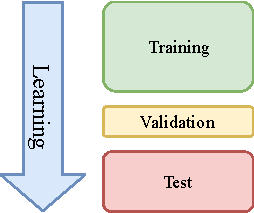
\includegraphics[width=0.8\linewidth]{learning.pdf}
		\caption{Learning}
	\end{subfigure}
	\begin{subfigure}[t]{0.48\linewidth}
		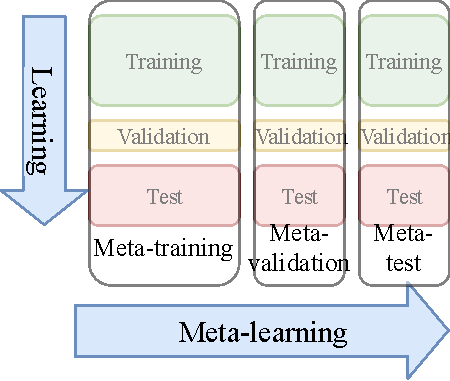
\includegraphics[width=0.8\linewidth]{meta_learning.pdf}
		\caption{Meta-learning}
	\end{subfigure}
\end{figure}
\end{frame}

